\chapter{Fondamenti di Machine Learning e Classificazione Classica}
\label{cap:fondamenti_ml_classificazione_classica}

Il Machine Learning (ML) rappresenta una branca fondamentale dell'Intelligenza Artificiale (AI), incentrata sullo sviluppo di algoritmi capaci di identificare autonomamente pattern complessi e regolarità all'interno dei dati. A differenza della programmazione imperativa tradizionale, in cui le regole logiche vengono esplicitamente codificate, il paradigma del ML apprende tali regole mediante un processo di ottimizzazione guidato dall'esperienza empirica\footnote{Mitchell, T. M. (1997). \textit{Machine Learning}. McGraw-Hill, New York.}.

Questo capitolo stabilisce il quadro teorico, matematico e metodologico del Machine Learning e della classificazione classica, con l'obiettivo di definire le basi prestazionali necessarie per il successivo confronto con i modelli di Quantum Machine Learning (QML). Nello specifico, verranno formalizzati i paradigmi di apprendimento, la formulazione matematica del problema di classificazione, le fasi di pre-processing fondamentali per il trattamento di dataset reali, i modelli di classificazione di riferimento (Logistic Regression, Support Vector Machines e Random Forest) e il rigoroso impianto metrico per la loro valutazione. \\

% \clearpage

\section{Paradigmi di Apprendimento}

L'apprendimento automatico si articola in tre paradigmi fondamentali, definiti dalla natura del feedback ricevuto nella fase di training (apprendimento supervisionato, non supervisionato e per rinforzo).

\subsection{Apprendimento Supervisionato}
Nell'apprendimento supervisionato il modello viene addestrato utilizzando un dataset di addestramento con etichette. Ogni istanza nel dataset è composta da una coppia di input e da un'etichetta di riferimento corrispondente, nota come \textit{ground truth} ($x_i, y_i$). L'obiettivo principale dell'algoritmo è apprendere una funzione di mappatura $h: \mathcal{X} \to \mathcal{Y}$ capace di generalizzare correttamente su dati non visti in fase di training, minimizzando una funzione di perdita (\textit{loss function}) che quantifica l'errore commesso nelle previsioni.

Questo approccio trova principale applicazione in due macro-categorie di problemi:
\begin{itemize}
    \item \textbf{Classificazione:} L'obiettivo è assegnare l'input $x$ a una categoria appartenente a un insieme discreto e finito di classi (es. riconoscimento di immagini, filtrazione di email spam). La variabile target $y$ assume valori in un insieme di etichette categoriali.
    \item \textbf{Regressione:} L'obiettivo è predire un valore continuo appartenente all'insieme dei numeri reali $y \in \mathbb{R}$ (es. previsione del prezzo di un immobile). La bontà del modello viene comunemente valutata tramite metriche come l'errore quadratico medio (\textit{Mean Squared Error}, MSE):
    \begin{equation}
        \text{MSE} = \frac{1}{n}\sum_{i=1}^n (y_i - \hat{y}_i)^2,
    \end{equation}
    dove $y_i$ è il valore reale e $\hat{y}_i$ è il valore predetto dal modello per l'$i-esimo$ campione.
\end{itemize}

\begin{figure}[htbp]
    \centering
    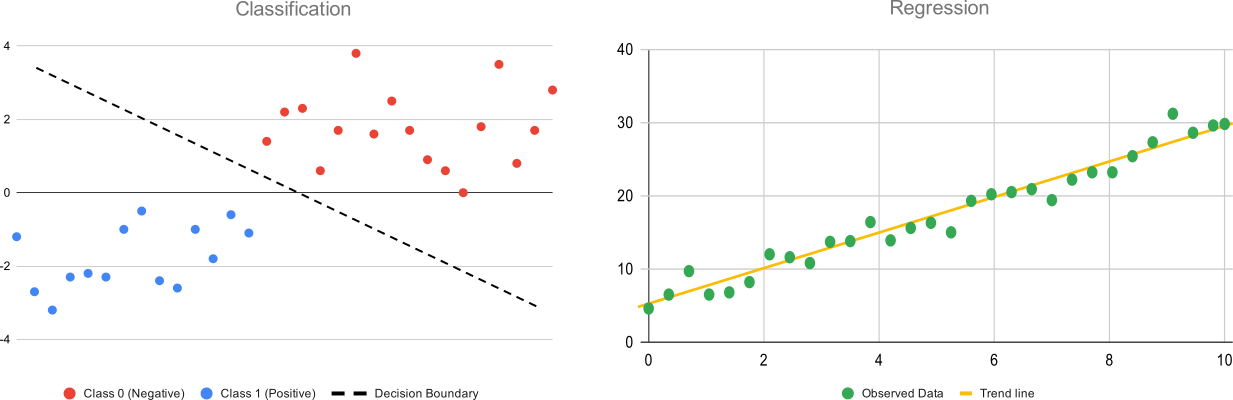
\includegraphics[width=1\textwidth]{assets/classification_vs_regression.png}
    \caption{\footnotesize Rappresentazione schematica del flusso di lavoro dell'Apprendimento Supervisionato, suddiviso nei compiti di Classificazione (output categoriale) e Regressione (output numerico continuo).}
    \label{fig:apprendimento_supervisionato}
\end{figure}

\subsection{Apprendimento Non Supervisionato}
Nell'apprendimento non supervisionato il dataset è composto unicamente dai vettori di input $\mathbf{x}_i \in \mathbb{R}^d$ (per $i = 1, \dots, n$), senza etichette di riferimento: non essendoci una \textit{ground truth} a fare da guida, l'algoritmo deve esplorare in autonomia la geometria dei dati per far emergere pattern nascosti, densità di probabilità o raggruppamenti spontanei.

Le metodologie chiave si articolano principalmente in due aree:

\begin{itemize}
    \item \textbf{Clustering:} Consiste nel partizionamento dello spazio dei tratti in cluster omogenei, in modo che gli elementi dello stesso gruppo siano altamente simili tra loro (\textit{alta coesione interna}) e nettamente dissimili da quelli di altri gruppi (\textit{alta separazione esterna}). Algoritmi come il $K$-Means minimizzano iterativamente la sommatoria delle distanze quadratiche all'interno dei cluster (\textit{inerzia}):
    \begin{equation}
        J = \sum_{j=1}^{K} \sum_{\mathbf{x}_i \in S_j} \|\mathbf{x}_i - \boldsymbol{\mu}_j\|^2,
    \end{equation}
    dove $S_j$ è il sottoinsieme di punti assegnati al cluster $j$-esimo e $\boldsymbol{\mu}_j$ il relativo centroide. Altri approcci rilevanti includono DBSCAN, basato sulla densità, e il clustering gerarchico.

    \item \textbf{Riduzione della Dimensionalità:} Proietta i dati da uno spazio ad alta dimensionalità $d$ a uno spazio a bassa dimensionalità $k$ (con $k \ll d$), contrastando la ``maledizione della dimensionalità'' (\textit{curse of dimensionality}) e alleggerendo il carico computazionale senza distruggere le informazioni chiave del dataset. Sul fronte lineare lo strumento d'elezione è l'Analisi delle Componenti Principali (\textit{PCA}), trattata più avanti in questo capitolo; per varietà non lineari (\textit{manifolds}) si impiegano algoritmi come t-SNE e UMAP.
\end{itemize}

\vfill

\begin{figure}[htbp]
    \centering
    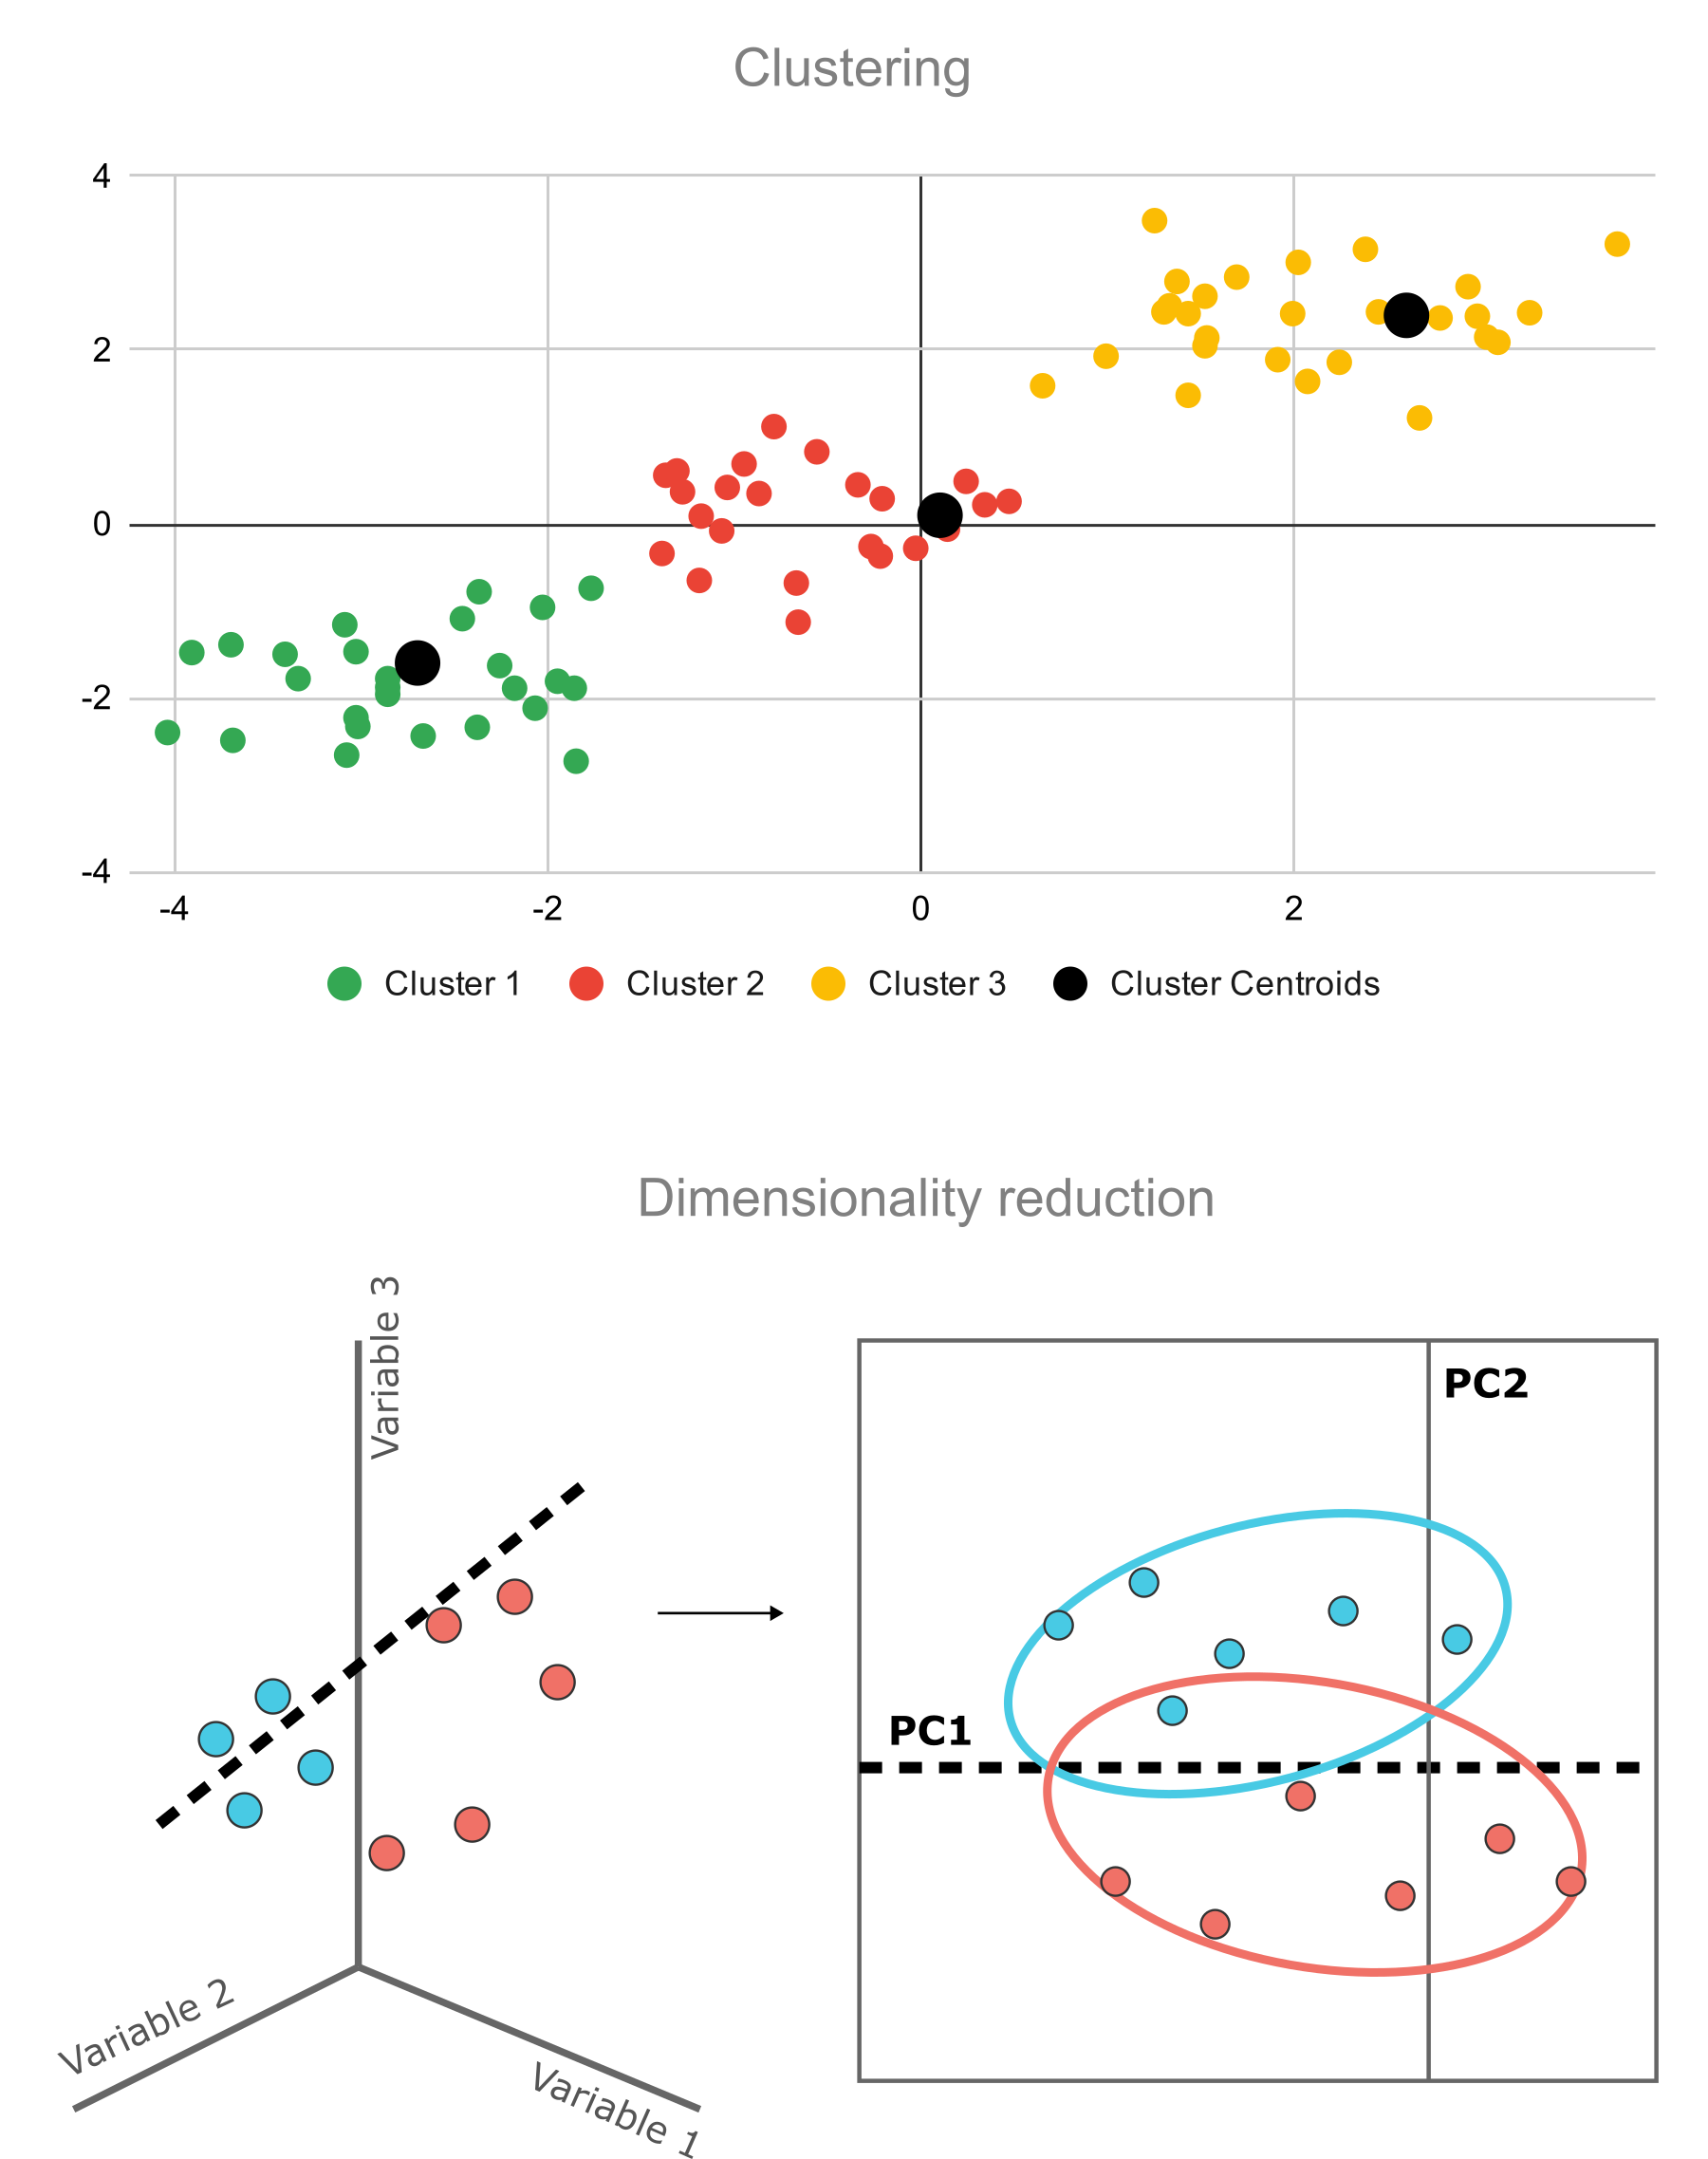
\includegraphics[width=0.5\textwidth]{assets/clustering_vs_dimensionality_reduction.png}
    \caption{\footnotesize Illustrazione dei compiti principali dell'Apprendimento Non Supervisionato: raggruppamento di dati simili in sottoinsiemi distinti (Clustering) e compressione geometrica dello spazio dei tratti (Riduzione della Dimensionalità).}
    \label{fig:apprendimento_non_supervisionato}
\end{figure}

\subsection{Apprendimento per Rinforzo}
L'Apprendimento per Rinforzo (\textit{Reinforcement Learning}, RL) si focalizza sull'apprendimento orientato ad un obiettivo. A differenza dei paradigmi supervisionati e non supervisionati, l'agente non impara da un dataset statico, ma apprende attraverso l'esperienza diretta derivante dall'interazione continua tra un agente razionale e un ambiente stocastico, dinamico e inizialmente sconosciuto, formalizzata matematicamente mediante il Processo Decisionale di Markov (\textit{Markov Decision Process}, MDP)\footnote{Sutton, R. S., \& Barto, A. G. (2018). \textit{Reinforcement Learning: An Introduction}. MIT Press.}: a ogni istante temporale discreto l'agente percepisce lo stato corrente dell'ambiente, seleziona ed esegue un'azione in base alla propria politica, transita a un nuovo stato e riceve un segnale di ricompensa numerico.

L'obiettivo dell'agente consiste nel determinare una politica ottimale in grado di massimizzare il valore atteso del ritorno cumulativo scontato nel lungo periodo, tipicamente stimato tramite funzioni di valore ottimizzate risolvendo l'equazione di ottimalità di Bellman. I principali approcci per la risoluzione di questo problema includono metodi basati su tabelle come il \textit{Q-Learning} e il \textit{SARSA}, fino ad arrivare ad algoritmi di \textit{Deep Reinforcement Learning} (es. DQN, PPO) che impiegano reti neurali profonde come approssimatori di funzione per gestire spazi di stato ad altissima dimensionalità.

\begin{figure}[htbp]
    \centering
    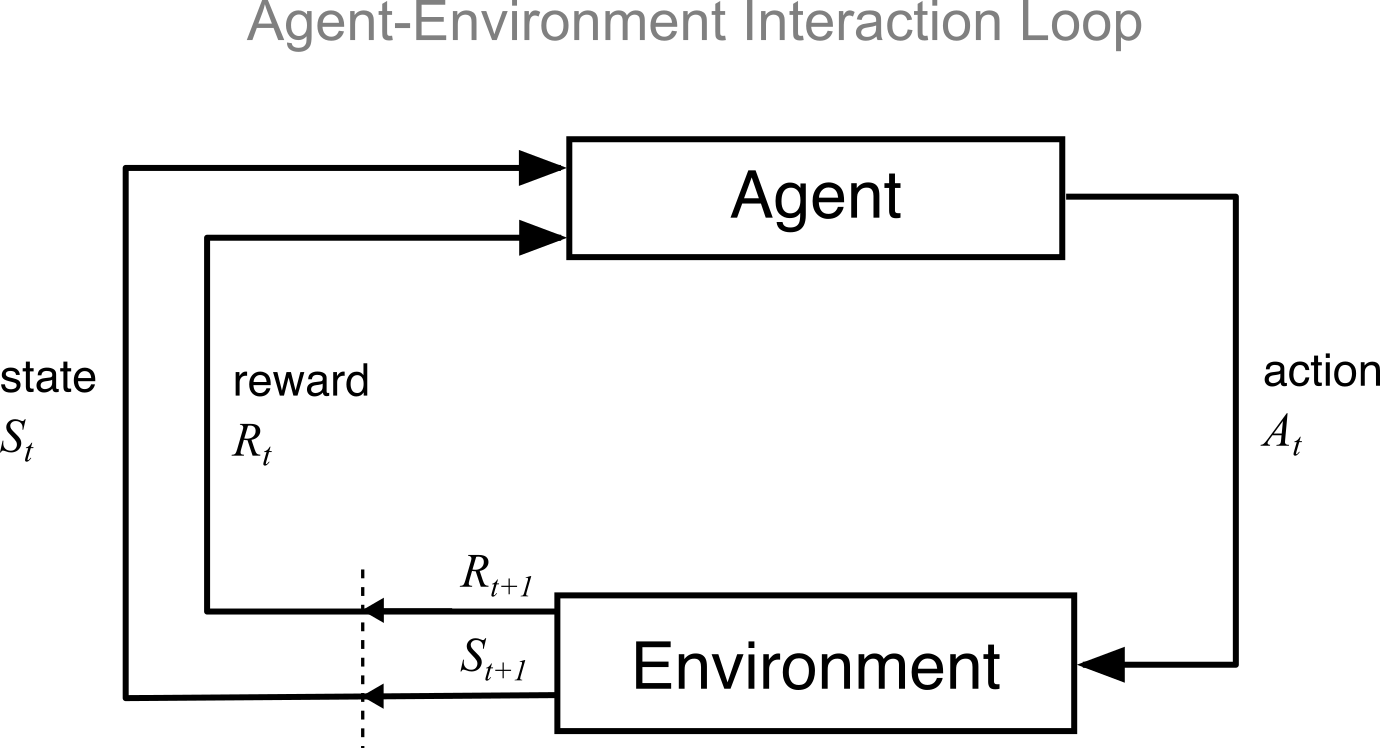
\includegraphics[width=0.60\textwidth]{assets/markov_decision_processes.png}
    \caption{\footnotesize Diagramma del ciclo di interazione Agente-Ambiente nel processo decisionale di Markov: l'agente esegue un'azione condizionata dallo stato corrente e riceve in risposta dall'ambiente un nuovo stato e una ricompensa scalare.}
    \label{fig:apprendimento_rinforzo_ciclo}
\end{figure}

\subsection{Dilemma Bias-Varianza, Overfitting e Underfitting}
La capacità di un modello di apprendimento di generalizzare su dati non visti è governata dal fondamentale compromesso tra errore di distorsione (\textit{Bias}) ed errore di varianza (\textit{Variance})\footnote{Hastie, T., Tibshirani, R., \& Friedman, J. (2009). \textit{The Elements of Statistical Learning}. Springer.}.

Considerando un problema di regressione con funzione di perdita quadratica, l'errore di generalizzazione atteso per un estimatore $\hat{f}(\mathbf{x})$ si scompone analiticamente nella somma di tre componenti chiave:
\begin{equation}
\mathbb{E}\left[(y - \hat{f}(\mathbf{x}))^2\right] = \text{Bias}\left[\hat{f}(\mathbf{x})\right]^2 + \text{Var}\left[\hat{f}(\mathbf{x})\right] + \sigma^2_{\epsilon},
\end{equation}
dove $\sigma^2_{\epsilon}$ rappresenta il rumore irriducibile intrinseco alla distribuzione dei dati.
I due errori più comuni dell'apprendimento sono:

\begin{itemize}
    \item \textbf{Underfitting (Alto Bias):} Si manifesta quando il modello possiede una capacità espressiva insufficiente per catturare la complessità strutturale sottostante ai dati. Un esempio classico è l'impiego di un regressore lineare per approssimare relazioni fortemente non lineari, il che si traduce in un errore sistematico elevato sia sul set di training che su quello di test.
    \item \textbf{Overfitting (Alta Varianza):} Si verifica quando la complessità del modello è eccessiva rispetto alla numerosità o alla qualità del dataset. In questo scenario, il modello finisce per apprendere e memorizzare il rumore specifico del set di addestramento anziché il pattern generale, compromettendo drasticamente le performance di generalizzazione.
\end{itemize}

Nel contesto del Machine Learning Quantistico, la gestione di questo trade-off assume peculiarità rilevanti: i circuiti quantistici parametrizzati (PQC) possono mostrare uno spazio delle ipotesi estremamente ampio ma, al contempo, rischiare fenomeni di overfitting accelerato o problemi di ottimizzazione legati alla geometria dello spazio degli stati (come il fenomeno dei \textit{barren plateaus})\footnote{Cerezo, M., et al. (2021). Cost function dependent barren plateaus in shallow quantum neural networks. \textit{Nature Communications}, 12(1), 1791.}.

\begin{figure}[htbp]
    \centering
    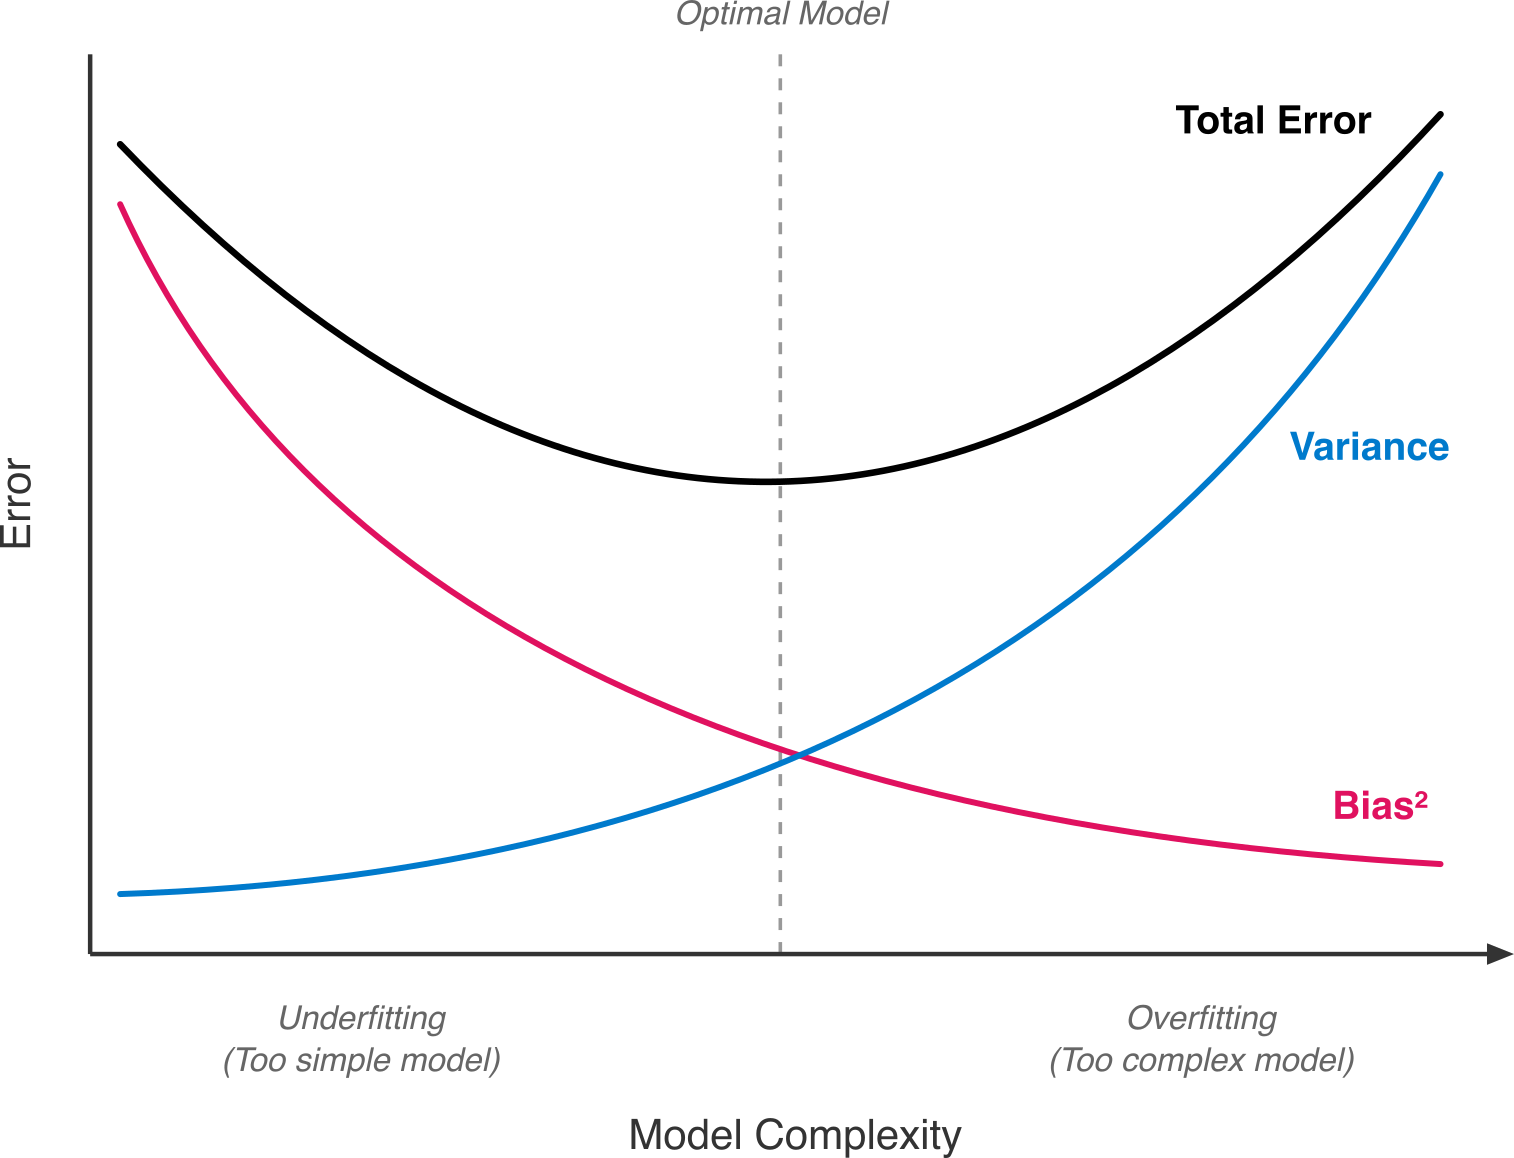
\includegraphics[width=0.65\textwidth]{assets/bias_variance_tradeoff.png}
    \caption{\footnotesize Decomposizione Bias-Varianza ed evoluzione dell'errore al variare della complessità del modello. La curva dell'errore totale mostra il tipico andamento a U, identificando il punto di ottimo (\textit{sweet spot}) tra l'underfitting (alto bias) e l'overfitting (alta varianza).}
    \label{fig:bias_variance_tradeoff}
\end{figure}

\section{Formulazione Matematica della Classificazione Supervisionata}

Focalizzando l'attenzione sul paradigma dell'apprendimento supervisionato, in questa sezione si formalizza il problema della classificazione binaria e multiclasse. Sia $\mathcal{X} \subseteq \mathbb{R}^d$ lo spazio dei tratti (\textit{feature space}) di dimensione $d$, e sia $\mathcal{Y}$ lo spazio discreto delle etichette di classe: nel caso binario $\mathcal{Y} = \{-1, +1\}$ oppure $\{0, 1\}$, nel caso multiclasse con $K$ categorie $\mathcal{Y} = \{1, 2, \dots, K\}$. Un dataset di addestramento $\mathcal{D} = \{(\mathbf{x}_i, y_i)\}_{i=1}^{n} \subset \mathcal{X} \times \mathcal{Y}$ è composto da $n$ coppie indipendenti e identicamente distribuite (i.i.d.), estratte da una distribuzione di probabilità congiunta sconosciuta $\mathcal{P}(\mathbf{X}, Y)$.

L'obiettivo dell'algoritmo di apprendimento è determinare una funzione $f: \mathcal{X} \to \mathcal{Y}$ che minimizzi l'errore atteso di predizione, quantificato da una funzione di perdita (\textit{loss function}). Poiché la distribuzione $\mathcal{P}$ è ignota, tale errore viene approssimato in pratica calcolandolo sul solo insieme di addestramento disponibile (\textit{Empirical Risk Minimization})\footnote{Vapnik, V. N. (1998). \textit{Statistical Learning Theory}. Wiley, New York.}, tipicamente aggiungendo un termine di regolarizzazione che penalizza la complessità del modello per prevenire l'overfitting.

\subsection{Funzioni di Perdita Principali}
La scelta della funzione di perdita dipende dall'algoritmo: la SVM (Sezione~\ref{sec:svm_classica}) utilizza tipicamente la \textit{Hinge Loss} per massimizzare il margine, mentre la Regressione Logistica impiega la \textbf{Binary Cross-Entropy} (o \textit{Logarithmic Loss}):
\begin{equation}
L_{\text{log}}(\hat{p}, y) = - \left[ y \log(\hat{p}) + (1 - y) \log(1 - \hat{p}) \right],
\end{equation}
dove $\hat{p} = P(Y=1 | \mathbf{X}=\mathbf{x})$ è la probabilità stimata dal modello; nel caso multiclasse si generalizza nella \textit{Categorical Cross-Entropy}.

\section{Preprocessing dei Dati per Dataset Reali}
I dataset del mondo reale presentano intrinsecamente problematiche di rumore, disomogeneità di scala e alta dimensionalità. La fase di preparazione è cruciale sia per la stabilizzazione della convergenza nei modelli classici, sia per consentire una corretta codifica dei dati all'interno dei registri quantistici.

\subsection{Normalizzazione e Ridimensionamento delle Caratteristiche}

Gli algoritmi basati sulla distanza (SVM, $k$-NN) e gli algoritmi basati sull'ottimizzazione (Regressione Logistica) sono molto sensibili alle differenze di scala nelle variabili. Per questo la scelta del metodo di ridimensionamento è fondamentale in quanto quanto una scelta sbagliata può influenzare significativamente l'efficienza e la coerenza dell'algoritmo.
Nel caso degli algoritmi quantistici, inoltre, un ridimensionamento sbagliato distorce l'encoding dei dati.

\begin{itemize}
    \item \textbf{Standardizzazione (Z-score Scaling):} Centra la variabile a media nulla e varianza unitaria ($\mu = 0$, $\sigma^2 = 1$):
    \begin{equation}
    x_{ij}' = \frac{x_{ij} - \mu_j}{\sigma_j}.
    \end{equation}
    \item \textbf{Min-Max Scaling:} Mappa i valori nell'intervallo compatto $[0, 1]$ (oppure $[-\pi, \pi]$, intervallo particolarmente vantaggioso per il \textit{quantum feature mapping} mediante gate di rotazione quantistica):
    \begin{equation}
    x_{ij}' = \frac{x_{ij} - \min(x_j)}{\max(x_j) - \min(x_j)}.
    \end{equation}
\end{itemize}

\subsection{Riduzione della Dimensionalità: Principal Component Analysis (PCA)}
La riduzione della dimensionalità riveste un'importanza fondamentale nei progetti di Quantum Machine Learning eseguiti su architetture NISQ (\textit{Noisy Intermediate-Scale Quantum}), a causa delle attuali limitazioni fisiche sul numero di qubit disponibili e sulla profondità dei circuiti. Questa operazione non si limita a semplificare la struttura dei dati, ma costituisce il ponte logico necessario per mappare lo spazio delle feature classiche in uno spazio di stato quantistico compatibile con le risorse computazionali.

La PCA è una trasformazione ortogonale lineare che proietta i dati $\mathbf{X} \in \mathbb{R}^{n \times d}$ in un sottospazio a $k$ dimensioni ($k < d$), massimizzando la varianza dei dati proiettati.

Matematicamente, data la matrice di covarianza campionaria $\boldsymbol{\Sigma} = \frac{1}{n-1} \mathbf{X}^T \mathbf{X}$ (assumendo dati preventivamente centrati a media nulla), si risolve il problema agli autovalori:
\begin{equation}
\boldsymbol{\Sigma} \mathbf{v}_i = \lambda_i \mathbf{v}_i, \quad i=1, \dots, d,
\end{equation}
dove $\lambda_1 \geq \lambda_2 \geq \dots \geq \lambda_d \geq 0$ sono gli autovalori e $\mathbf{v}_i$ gli autovettori ortonormali associati.
Scegliendo i primi $k$ autovettori associati ai $k$ autovalori maggiori definiamo la matrice di proiezione $\mathbf{W}_k \in \mathbb{R}^{d \times k}$, utilizzando la quale calcoliamo il dataset ridotto $\mathbf{Z} = \mathbf{X} \mathbf{W}_k$.

\section{Algoritmi di Classificazione Classica di Benchmark}
\label{sec:algoritmi_classificazione_classica}

In questa sezione vengono introdotti i tre algoritmi selezionati come strumenti di confronto per un'analisi comparativa. La scelta di questi modelli in particolare non è arbitraria e le ragioni che la sostengono includono diversi fattori storici e pratici.

\subsection{Logistic Regression}
La Logistic Regression è un modello probabilistico lineare utilizzato per problemi di classificazione binaria. La probabilità a posteriori che un esempio $\mathbf{x}$ appartenga alla classe positiva $y=1$ è modellata tramite la funzione sigmoidale (o operatore logistico) $\sigma(z)$:
\begin{equation}
P(Y=1 | \mathbf{X}=\mathbf{x}) = \sigma(\mathbf{w}^T \mathbf{x} + b) = \frac{1}{1 + e^{-(\mathbf{w}^T \mathbf{x} + b)}},
\end{equation}
dove $\mathbf{w} \in \mathbb{R}^d$ è il vettore dei pesi e $b \in \mathbb{R}$ è il bias.

La storia della regressione logistica risale al lavoro di Ronald Fisher negli anni '30, e successivamente è stata sviluppata e formalizzata da statistici come David Cox negli anni '50. La sua eleganza matematica e la sua efficienza computazionale ne fanno uno standard riconosciuto per il controllo base dei modelli di classificazione. La funzione di costo è strettamente convessa, garantendo un punto di minimo globale unico e una convergenza rapida. Questo comportamento la rende particolarmente adatta come baseline che può essere facilmente confrontata con modelli più complessi.

L'ottimizzazione dei parametri avviene massimizzando la funzione di Log-verosimiglianza (\textit{Log-likelihood}):
\begin{equation}
\ell(\mathbf{w}, b) = \sum_{i=1}^{n} \left[ y_i \log \sigma(\mathbf{w}^T \mathbf{x}_i + b) + (1-y_i) \log (1 - \sigma(\mathbf{w}^T \mathbf{x}_i + b)) \right].
\end{equation}
La minimizzazione della perdita equivale a minimizzare la Cross-Entropy negativa. Poiché la funzione di costo è strettamente convessa, il punto di minimo globale può essere raggiunto in modo efficiente mediante algoritmi di ottimizzazione quasi-Newtoniani come L-BFGS o mediante Stochastic Gradient Descent (SGD).

\begin{figure}[htbp]
    \centering
    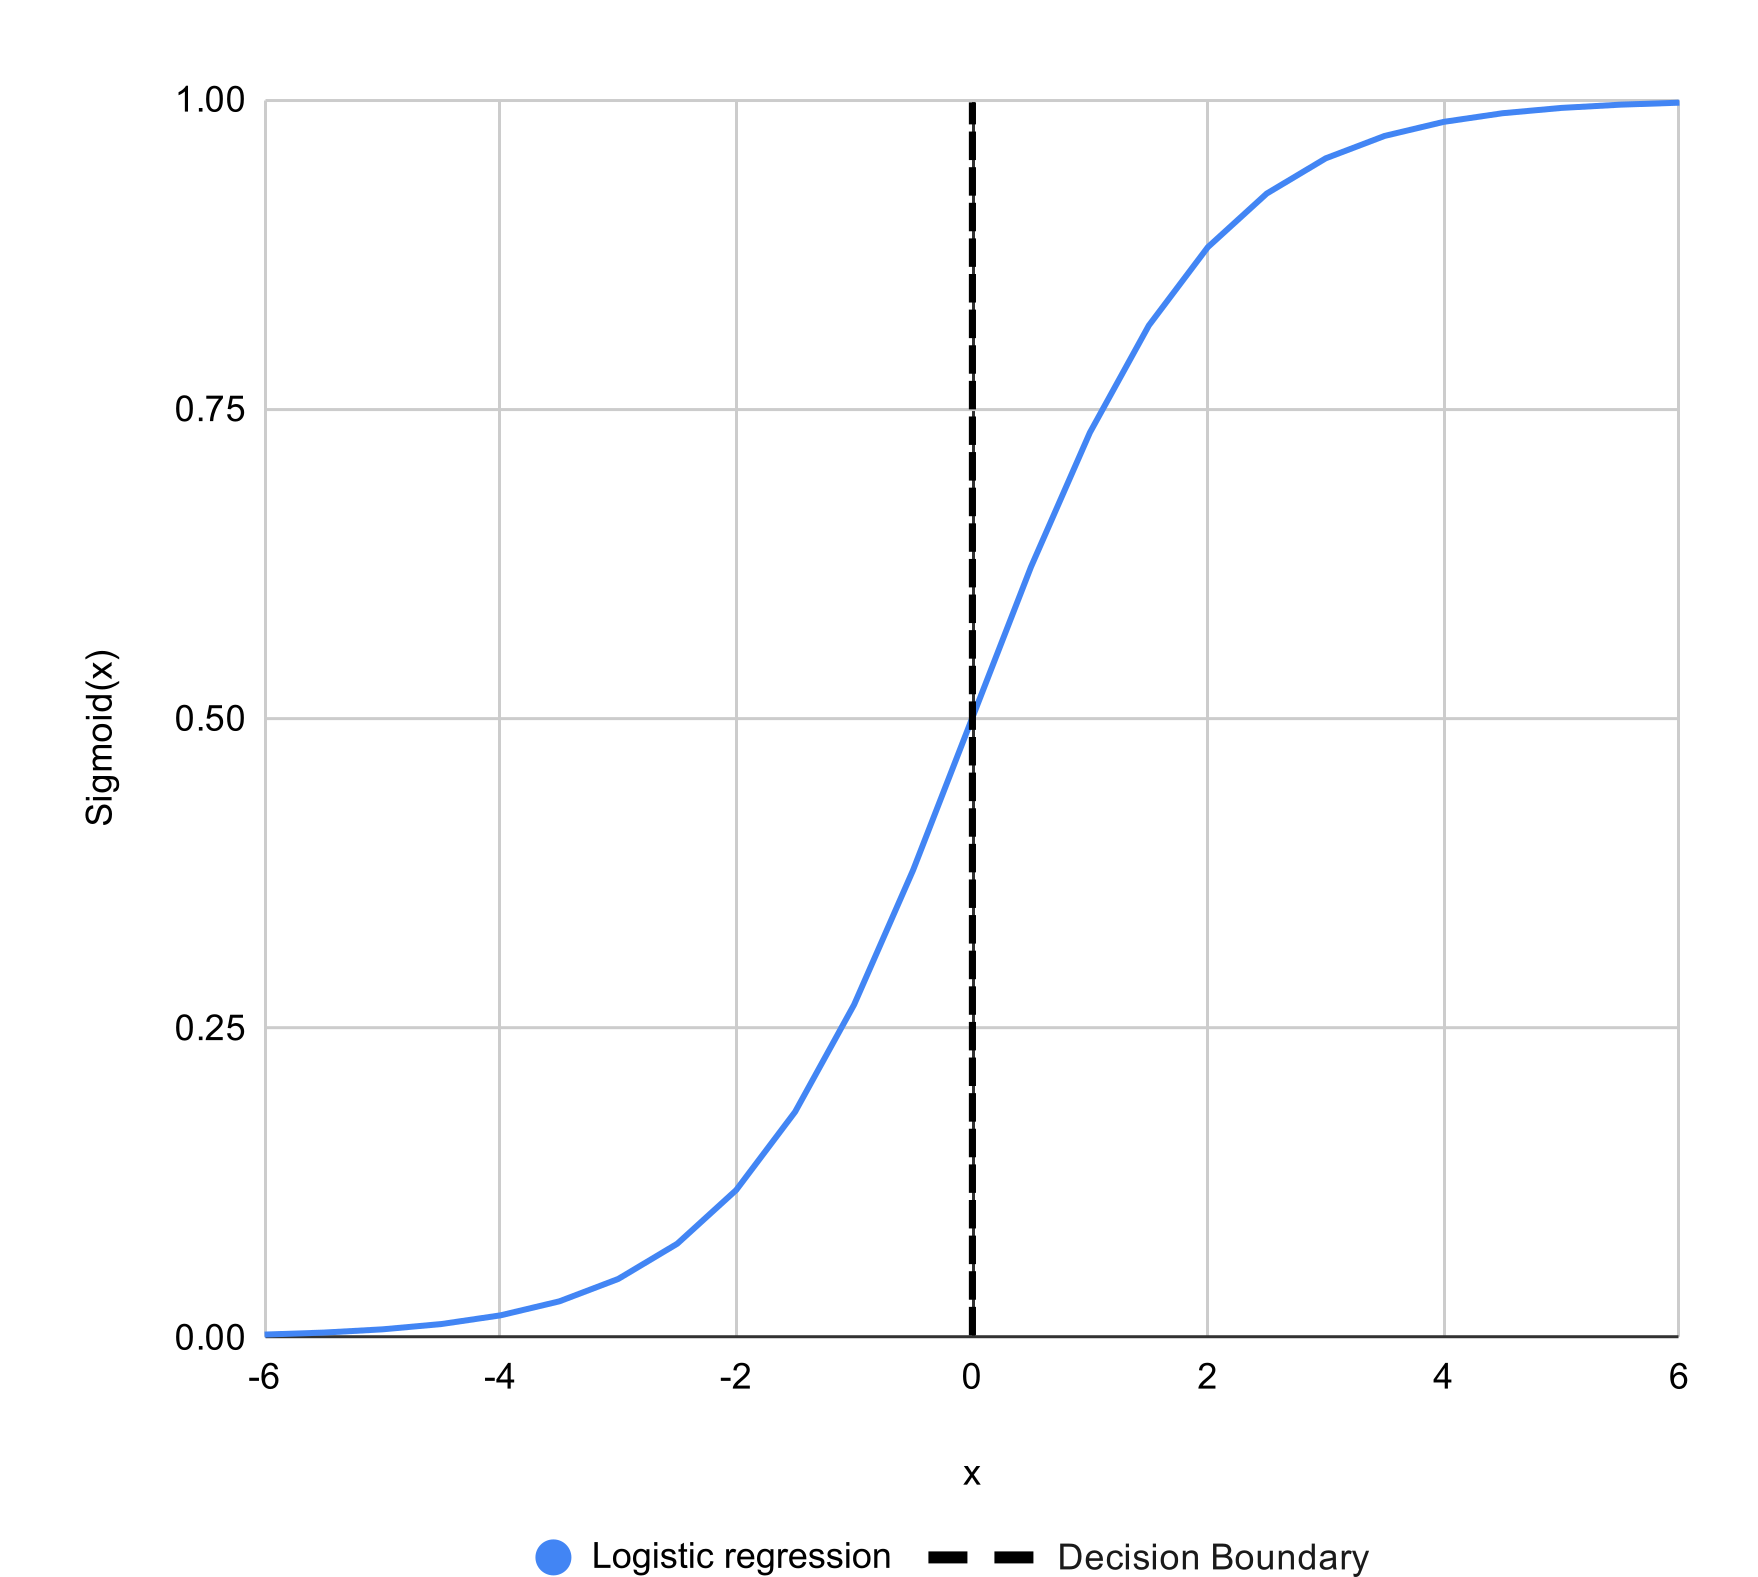
\includegraphics[width=0.60\textwidth]{assets/logistic_regression.png}
    \caption{\footnotesize Rappresentazione della funzione di attivazione sigmoidea utilizzata nella regressione logistica, che mappa i valori di input (x) alle probabilità di output.}
    \label{fig:funzione_sigmoidale}
\end{figure}

\subsection{Support Vector Machines (SVM)}
\label{sec:svm_classica}
Le Support Vector Machines rappresentano uno dei modelli di classificazione a margine massimo più rigorosi dal punto di vista teorico. Questo modello è stato introdotto da Vladimir Vapnik durante la sua ricerca nel campo della teoria statistica dell'apprendimento negli anni '60, con una formalizzazione completa negli anni '90.

La formulazione teorica ha profonde basi matematiche: il problema di ottimizzazione è fondato su principi di programmazione convessa e ha una soluzione unica grazie al teorema della dualità. Il concetto di margine massimo fornisce un'interpretazione geometrica chiara delle capacità generalizzative dei modelli: il margine più ampio tra le classi indica una maggiore separabilità dei dati.

\subsubsection{Formulazione Primal e Margine Ampio}
Dato un set di addestramento linearmente separabile con $y_i \in \{-1, +1\}$, l'obiettivo è individuare un iperpiano di decisione $\mathbf{w}^T \mathbf{x} + b = 0$ che separi le classi massimizzando il margine geometrico $\frac{2}{\|\mathbf{w}\|_2}$.

In presenza di dati non perfettamente separabili, si introduce una penalizzazione per le violazioni del margine mediante le variabili di \textit{slack} $\xi_i \ge 0$ (Formulazione Soft-Margin). Il problema di ottimizzazione primale si esprime come:
\begin{equation}
\begin{aligned}
\min_{\mathbf{w}, b, \boldsymbol{\xi}} \quad & \frac{1}{2} \|\mathbf{w}\|^2 + C \sum_{i=1}^{n} \xi_i \\
\text{s.t.} \quad & y_i (\mathbf{w}^T \mathbf{x}_i + b) \ge 1 - \xi_i, \quad \forall i=1, \dots, n \\
& \xi_i \ge 0, \quad \forall i=1, \dots, n,
\end{aligned}
\end{equation}
dove $C > 0$ è un iperparametro di regolarizzazione che governa il compromesso tra l'ampiezza del margine e le violazioni ammesse.

\subsubsection{Formulazione Duale di Wolfe e Kernel Trick}
Applicando i moltiplicatori di Lagrange $\alpha_i \ge 0$ e $\mu_i \ge 0$, la funzione Lagrangiana è:
\begin{equation}
\mathcal{L}(\mathbf{w}, b, \boldsymbol{\xi}, \boldsymbol{\alpha}, \boldsymbol{\mu}) = \frac{1}{2} \|\mathbf{w}\|^2 + C \sum_{i=1}^n \xi_i - \sum_{i=1}^n \alpha_i \left[ y_i(\mathbf{w}^T \mathbf{x}_i + b) - 1 + \xi_i \right] - \sum_{i=1}^n \mu_i \xi_i.
\end{equation}
Annullando le derivate parziali rispetto alle variabili primali ($\mathbf{w}, b, \boldsymbol{\xi}$), si ottengono le condizioni di ottimalità Karush-Kuhn-Tucker (KKT):
\begin{equation}
\mathbf{w} = \sum_{i=1}^{n} \alpha_i y_i \mathbf{x}_i, \quad \sum_{i=1}^{n} \alpha_i y_i = 0, \quad C - \alpha_i - \mu_i = 0.
\end{equation}

\noindent Sostituendo tali relazioni nella Lagrangiana si ottiene la forma duale di Wolfe:
\begin{equation}
\begin{aligned}
\max_{\boldsymbol{\alpha}} \quad & \sum_{i=1}^{n} \alpha_i - \frac{1}{2} \sum_{i=1}^{n} \sum_{j=1}^{n} \alpha_i \alpha_j y_i y_j \langle \mathbf{x}_i, \mathbf{x}_j \rangle \\
\text{s.t.} \quad & 0 \le \alpha_i \le C, \quad \forall i=1, \dots, n \\
& \sum_{i=1}^{n} \alpha_i y_i = 0.
\end{aligned}
\end{equation}

\noindent I vettori per i quali $\alpha_i > 0$ sono definiti \textit{vettori di supporto} (\textit{support vectors}).

Nel caso di pattern non linearmente separabili nello spazio originale $\mathbb{R}^d$, si applica una mappatura non lineare $\Phi: \mathcal{X} \to \mathcal{F}$ in uno spazio di Hilbert ad alta (o infinita) dimensione $\mathcal{F}$. Grazie al \textbf{Kernel Trick}\footnote{Boser, B. E., Guyon, I. M., \& Vapnik, V. N. (1992). A training algorithm for optimal margin classifiers. \textit{Proceedings of the fifth annual workshop on Computational learning theory}, 144-152.}, non è necessario calcolare esplicitamente la trasformazione $\Phi(\mathbf{x})$, ma è sufficiente valutare la funzione kernel $K(\mathbf{x}_i, \mathbf{x}_j) = \langle \Phi(\mathbf{x}_i), \Phi(\mathbf{x}_j) \rangle_{\mathcal{F}}$.

Tra le funzioni Kernel classiche più ampie figura il Kernel Gaussiano a base Radiale (RBF):
\begin{equation}
K_{\text{RBF}}(\mathbf{x}_i, \mathbf{x}_j) = \exp\left( -\gamma \|\mathbf{x}_i - \mathbf{x}_j\|^2 \right), \quad \gamma > 0.
\end{equation}

\textit{Nota metodologica:} Il concetto di Kernel Trick applicato alle SVM costituisce l'esatto analogo matematico del \textit{Quantum Kernel Estimation} (QKE), in cui lo spazio delle caratteristiche $\mathcal{F}$ è sostituito dallo spazio degli stati di Hilbert dei qubit, e la mappa $\Phi(\mathbf{x})$ è implementata da un circuito quantistico parametrizzato.

\begin{figure}[htbp]
    \centering
    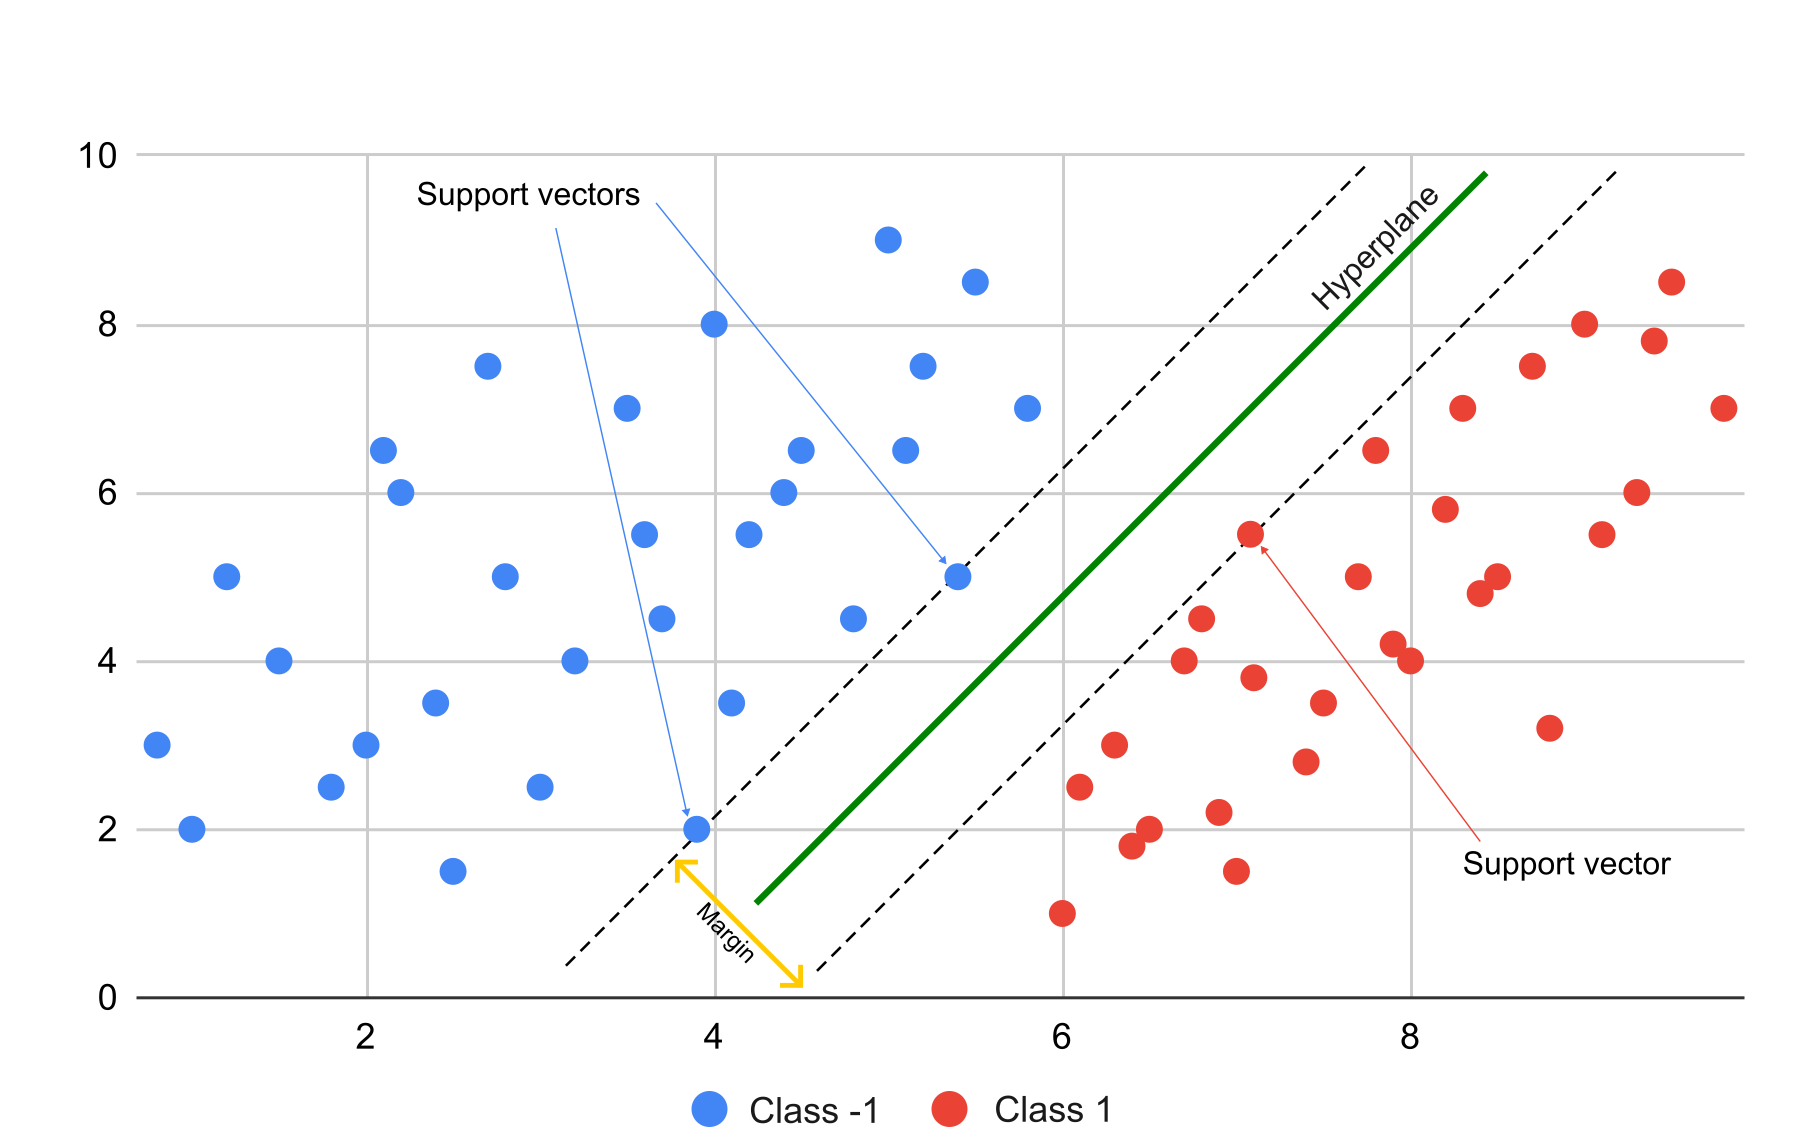
\includegraphics[width=0.7\textwidth]{assets/svm_hyperplane.png}
    \caption{\footnotesize Iperpiano di separazione e margine massimo in una Support Vector Machine.}
    \label{fig:svm_hyperplane}
\end{figure}

\subsection{Random Forest}
Il Random Forest\footnote{Breiman, L. (2001). Random Forests. \textit{Machine Learning}, 45(1), 5-32.} rappresenta dei più importanti esempi di algoritmi di apprendimento d'insieme (ensemble learning). Questo approccio è stato introdotto da Leo Breiman e Adele Cutler nel 2001, basandosi su principi già consolidati di \textit{Bootstrap Aggregating} (noto comunemente come \textit{bagging}).

L'approccio dell'ensemble si basa sull'idea che combinando modelli diversi si possa ottenere un miglioramento della capacità predittiva rispetto a quella di un singolo modello. L'unione di \textit{bagging} e alberi decisionali ha dimostrato una notevole robustezza e un'elevata capacità di generalizzazione, rendendo il Random Forest uno strumento standard ampiamente adottato in ambito ML.

\subsubsection{Algoritmo di Costruzione}
Per un ensemble composto da $B$ alberi decisionali:
\begin{enumerate}
    \item Per ogni albero $b = 1, \dots, B$:
    \begin{enumerate}
        \item Si estrae un campione bootstrap $\mathcal{D}_b$ di dimensione $n$ dal dataset originale $\mathcal{D}$ tramite campionamento con reinserimento.
        \item Si addestra un albero decisionale $T_b$ sul campione $\mathcal{D}_b$. In ogni nodo dell'albero, la scelta della migliore scissione (\textit{split}) non avviene su tutte le $d$ feature, ma su un sottoinsieme casuale di dimensione $m \ll d$ (tipicamente $m = \lfloor\sqrt{d}\rfloor$).
        \item L'albero viene fatto crescere fino a una profondità massima $d_{\max}$ o fino al raggiungimento di un numero minimo di campioni per foglia, senza applicare potatura (\textit{pruning}).
    \end{enumerate}
\end{enumerate}

La regola di decisione per un nuovo campione $\mathbf{x}$ nel caso della classificazione binaria/multiclasse si basa sul voto di maggioranza (\textit{majority voting}):
\begin{equation}
\hat{y} = \text{mode} \left\{ T_1(\mathbf{x}), T_2(\mathbf{x}), \dots, T_B(\mathbf{x}) \right\}.
\end{equation}

\subsubsection{Misure di Impurità}
La scissione nei nodi degli alberi decisionali avviene minimizzando una misura di impurità. Le metriche più comunemente impiegate sono:
\begin{itemize}
    \item \textbf{Indice di Impurità di Gini:}
    \begin{equation}
    I_G(p) = 1 - \sum_{k=1}^{K} p_k^2;
    \end{equation}
    \item \textbf{Entropia (Informazionale di Shannon):}
    \begin{equation}
    I_H(p) = -\sum_{k=1}^{K} p_k \log_2(p_k);
    \end{equation}
\end{itemize}
dove $p_k$ rappresenta la proporzione di campioni appartenenti alla classe $k$ presente nel nodo considerato.

\begin{figure}[htbp]
    \centering
    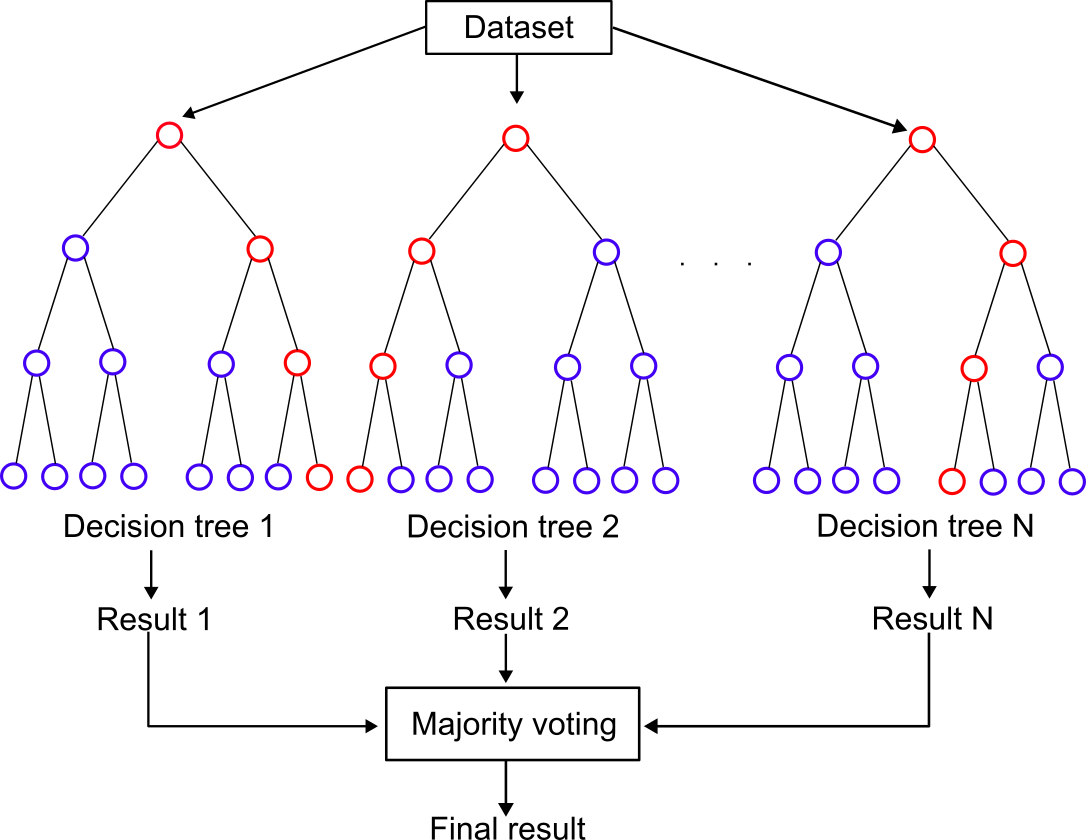
\includegraphics[width=0.7\textwidth]{assets/random_forest.png}
    \caption{\footnotesize Architettura ad albero combinato dell'algoritmo Random Forest.}
    \label{fig:random_forest}
\end{figure}

\section{Metodologia di Valutazione delle Prestazioni}

Per garantire un confronto oggettivo e statisticamente solido tra modelli classici e modelli quantistici, è necessario definire una metodologia di validazione rigorosa, capace di mitigare gli effetti della varianza statistica e dell'overfitting, insieme a un set esaustivo di metriche prestazionali.

\subsection{Partizionamento e Stratified $K$-Fold Cross-Validation}
\label{sec:partizionamento_kfold}
I dataset reali presentano frequentemente distribuzioni sbilanciate tra le classi. Un semplice \textit{hold-out split} casuale rischierebbe di produrre subset non rappresentativi della distribuzione originale, compromettendo l'affidabilità del test.

Si adotta pertanto la \textbf{Stratified $K$-Fold Cross-Validation}. Il dataset $\mathcal{D}$ viene suddiviso in $K$ partizioni disgiunte $\mathcal{D}_1, \dots, \mathcal{D}_K$ preservando in ciascuna la medesima distribuzione di classe del set originale. A ogni iterazione $k \in \{1, \dots, K\}$, il modello viene addestrato su $\mathcal{D} \setminus \mathcal{D}_k$ e validato su $\mathcal{D}_k$. La prestazione finale è calcolata come media aritmetica dei risultati ottenuti sui $K$ fold, riducendo la dipendenza dell'algoritmo dallo specifico split scelto\footnote{Hastie, T., Tibshirani, R., \& Friedman, J. (2009). \textit{The Elements of Statistical Learning: Data Mining, Inference, and Prediction}. Springer Science \& Business Media.}.

\subsection{Matrice di Confusione e Metriche di Classificazione}
Per quantificare l'errore del modello in problemi di classificazione binaria, si utilizza la matrice di confusione (Tab. \ref{tab:matrice_confusione}), dalla quale derivano gli indicatori fondamentali di prestazione:

\begin{table}[h]
\centering
\caption{Matrice di Confusione}
\label{tab:matrice_confusione}
\begin{tabular}{l|c|c}
\hline
& \textbf{Predetto Negativo ($Y=0$)} & \textbf{Predetto Positivo ($Y=1$)} \\
\hline
\textbf{Reale Negativo ($Y=0$)} & True Negative (TN) & False Positive (FP) \\
\textbf{Reale Positivo ($Y=1$)} & False Negative (FN) & True Positive (TP) \\
\hline
\end{tabular}
\end{table}

Oltre ad Accuracy, Precision, Recall e F1-Score, è essenziale considerare:
\begin{itemize}
    \item \textbf{Specificity (True Negative Rate):} $\text{TN} / (\text{TN} + \text{FP})$, fondamentale per bilanciare la Recall nei casi in cui l'identificazione dei negativi sia altrettanto critica dei positivi.
    \item \textbf{Matthews Correlation Coefficient (MCC):} Un indicatore più robusto dell'F1-Score, poiché tiene conto di tutti e quattro i quadranti della matrice di confusione, fornendo un valore di correlazione tra predizione e realtà tra -1 e +1.
\end{itemize}

\section{Limiti Computazionali dei Modelli Classici}

I modelli classici presentati in questo capitolo, per quanto efficaci sui dataset di dimensioni contenute utilizzati in questo lavoro, presentano vincoli computazionali intrinseci che ne limitano la scalabilità: la SVM a kernel non lineare (Sezione~\ref{sec:svm_classica}), ad esempio, richiede fino a $O(n^3 \cdot d)$ operazioni in fase di addestramento al crescere del numero di campioni $n$. Questi vincoli si accentuano ulteriormente quando si esplorano spazi di feature ad alto ordine per catturare correlazioni non lineari complesse (ad esempio tramite kernel polinomiali di grado elevato): il calcolo esplicito di tali feature comporta un'esplosione combinatoria che rende il problema rapidamente intrattabile, un fenomeno noto come \textit{Maledizione della Dimensionalità}\footnote{Bellman, R., \& Bellman, R. E. 1961, \textit{Adaptive Control Processes: A Guided Tour}. Princeton University Press.}.

È proprio questa limitazione a motivare l'interesse per il \textit{Quantum Feature Mapping}, discusso nel Capitolo~\ref{cap:quantum_machine_learning} (Sezione~\ref{sec:data_encoding}): mappando i dati in uno spazio di Hilbert di dimensione $2^N$ tramite $N$ qubit, i modelli quantistici accedono a spazi di feature ad altissima dimensionalità senza doverli costruire esplicitamente, aprendo potenziali vie per identificare regolarità nei dati che sfuggono ai modelli classici basati su distanze euclidee standard.